\section{SIEVE Design}
\subsection{Overview}
The overall framework of SIEVE consists of three stages, as illustrated in Figure~\ref{fig:4}.

\textbf{Stage I}: Nominal Inter-Layer Predictor Training. At each decoding step, SIEVE collects the last-token representation of the self-attention output projection (\texttt{o\_proj}) from the monitored decoder layers and reduces it to a low-dimensional space with a shared random orthogonal matrix. A layer-aware predictor is then trained on clean execution traces to learn the nominal mapping between adjacent monitored layers, providing a per-step runtime reference for subsequent discrepancy computation.

\textbf{Stage II}: Significant SDC Detector Training. Under fault injection configurations, the predictor trained in Stage I estimates the nominal downstream representation for each selected layer pair, which is paired with the actually observed representation during faulty execution. Over the first $K$ decoding steps, the cosine similarity, signed mean and standard-deviation differences, and L2 distance between the predicted and observed representations are aggregated into a Discrepancy Profile. Combined with semantic severity labels generated by an LLM Judge, these profiles are used to train a lightweight XGBoost detector that identifies SDCs significantly impacting the semantic output of the model.

\textbf{Stage III}: Online Significant SDC Detection. During actual deployment, only the trained Nominal Inter-Layer Predictor and the XGBoost detector are executed online, performing real-time Significant SDC detection from runtime intermediate features. Since the entire detection process requires neither additional fault-free inference nor substantial computational complexity, it effectively reduces runtime overhead while maintaining detection capability.

\begin{figure}[!ht]
\centering
    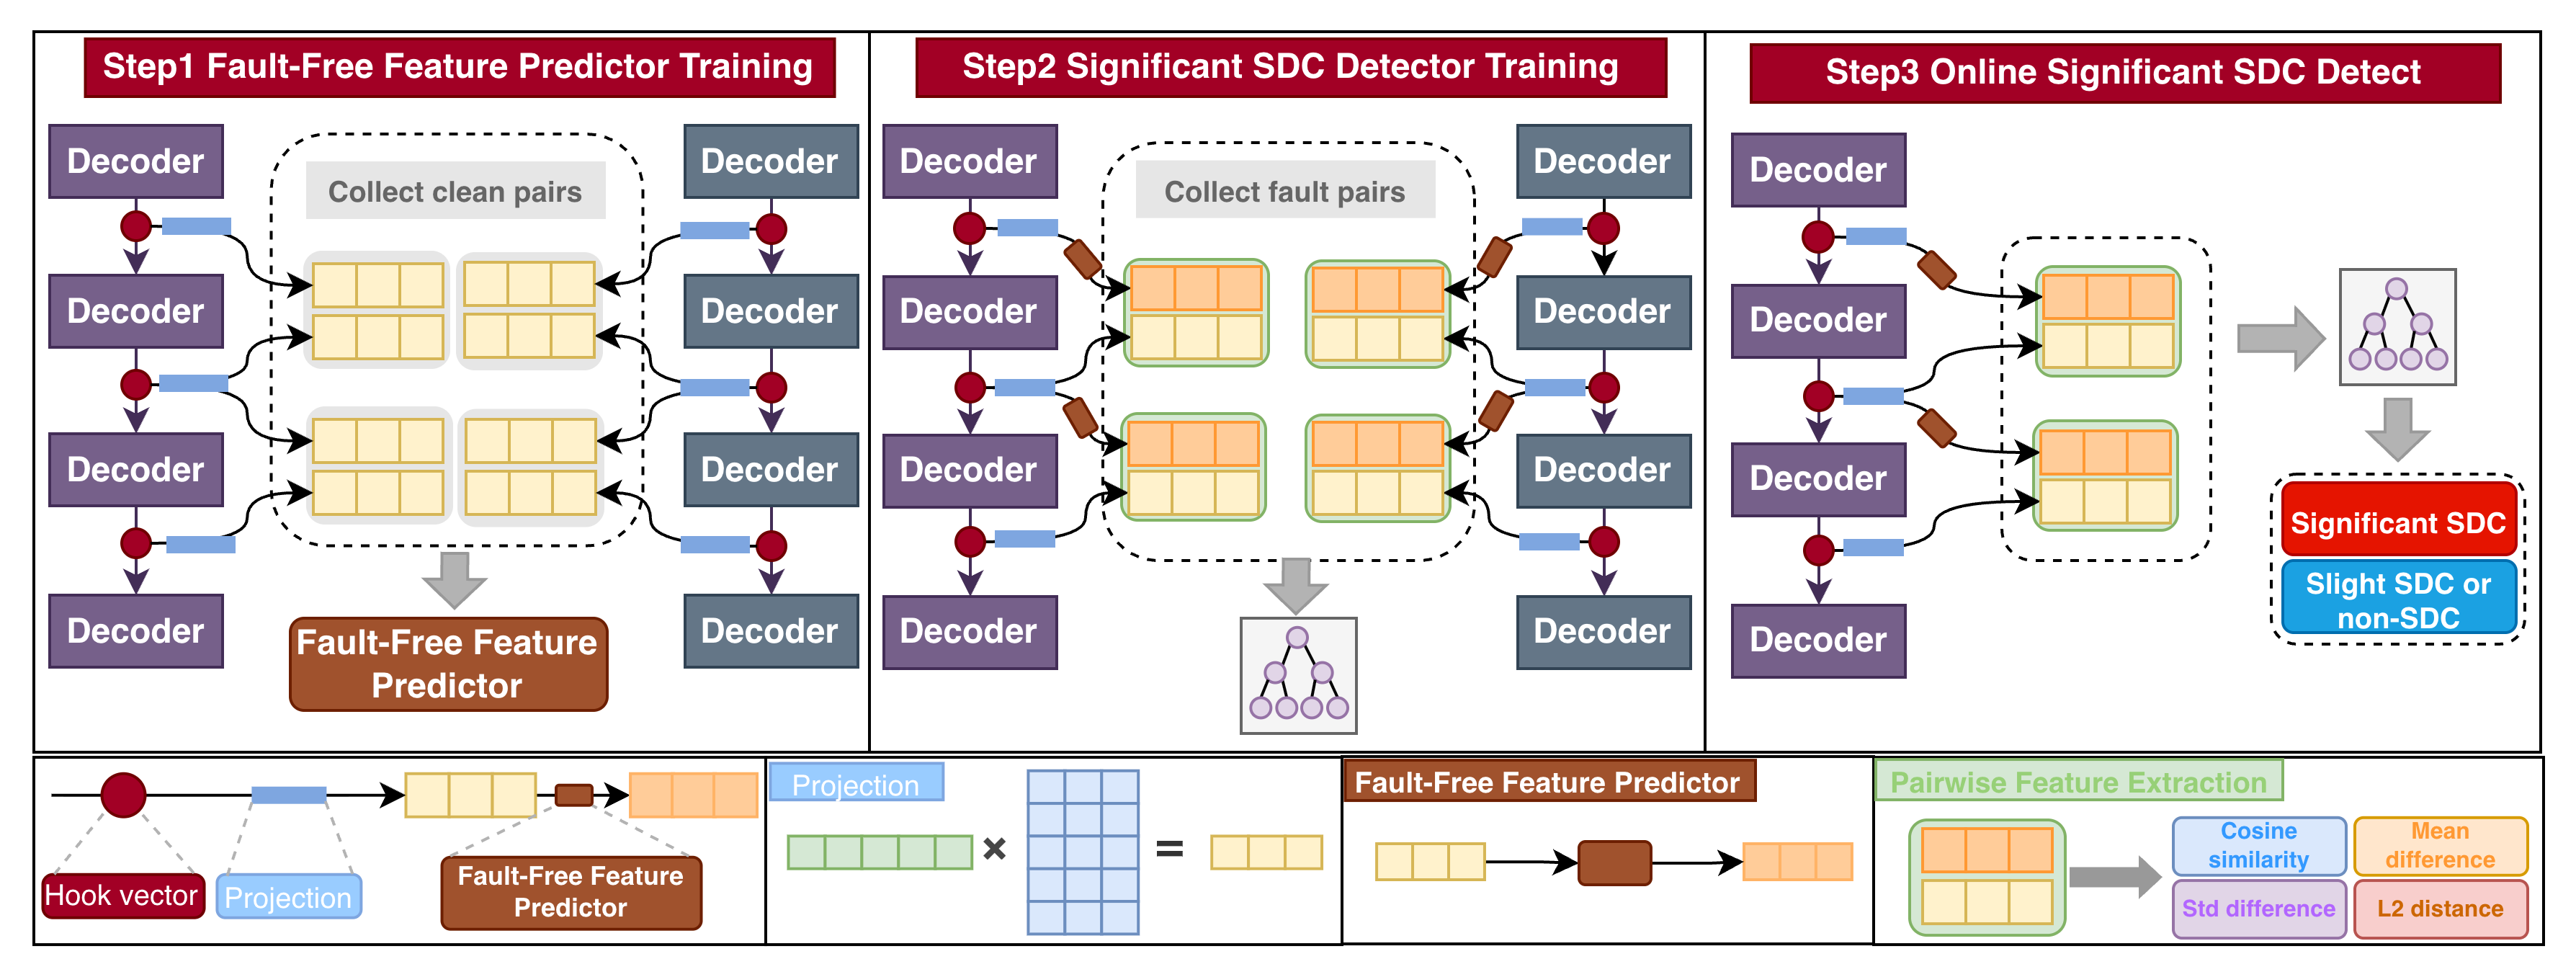
\includegraphics[width=1.0\linewidth]{Figures/figure4_SIEVE_overview.png}
    \caption{Overview of SIEVE. Per-layer attention outputs are projected to a low-dimensional space, a Nominal Inter-Layer Predictor models the nominal mapping between adjacent layers, and the resulting Discrepancy Profile feeds an XGBoost detector to flag Significant SDCs.}
    \label{fig:4}
\end{figure}

\subsection{Nominal Inter-Layer Predictor}
\subsubsection{Feature Collection}
To establish comparable reference features for runtime detection, we leverage PyTorch forward hooks to collect, at each decoding step of clean execution, the last-token representation of the self-attention output projection (\texttt{o\_proj}) of each monitored decoder layer, and organize adjacent monitored layers into feature pairs: the source-layer representation serves as the predictor's input while the target-layer representation acts as the supervision signal, learning the nominal inter-layer feature mapping. However, raw decoder features are extremely high-dimensional (e.g., 3,584 for Qwen2.5-VL-7B), making direct storage and training costly and increasing the difficulty of learning the mapping.

To this end, we project the features into a low-dimensional space. This design is inspired by the Johnson–Lindenstrauss (JL) lemma~\cite{johnson1984extensions}—random low-dimensional projections approximately preserve the geometric relations among samples—and employs a shared column-orthogonal projection matrix that maps features into a 64-dimensional space. Figure~\ref{fig:jl} (appendix) verifies this empirically via heatmaps of adjacent-layer relations and correlation scatter plots before and after projection: the reduced representations remain highly consistent with the original space, with Pearson and Spearman correlations of 0.909 and 0.902. The 64-dimensional projection thus preserves the dominant cross-layer geometric structure while substantially reducing both feature storage and predictor size.


\subsubsection{Predictor Training}
The predictor is trained to reconstruct the nominal feature of a target layer from the low-dimensional feature of its source layer. Since intermediate features require both element-wise numerical accuracy and the semantic consistency carried by their direction, supervising with Mean Squared Error (MSE) alone biases the model toward element-wise fidelity at the expense of directional consistency. We therefore adopt a combined objective. Let $\hat{\mathbf{Y}}$ denote the predictor's output and $\mathbf{Y}$ the corresponding nominal target feature; the training loss is
$$L = \alpha L_{\mathrm{mse}} + \beta L_{\mathrm{cos}}, \qquad L_{\mathrm{cos}} = 1 - \cos(\hat{\mathbf{Y}}, \mathbf{Y}),$$
where $\alpha$ and $\beta$ are hyperparameters that balance the two loss terms, both set to 1.0 in this work. The MSE term ensures numerical fidelity, while the cosine term constrains directional consistency in the representation space, yielding stable and semantically coherent predictions. Architecturally, the predictor is a layer-aware residual MLP: each 64-dimensional source feature is concatenated with a 16-dimensional layer embedding and passed through 8 residual blocks (hidden size 64, dropout 0.1) to produce the 64-dimensional nominal feature of the target layer, allowing a single shared network to distinguish the mapping of each monitored layer pair. After training, the predictor performs only one lightweight forward pass per step at runtime, and its output serves as the reference for the subsequent Discrepancy Profile.

\subsection{Significant SDC Detector Training}

\subsubsection{Discrepancy Profile}
To capture Significant-SDC signatures from the nominal reference features provided by the predictor, we construct a Discrepancy Profile that characterizes each predicted--actual feature pair from two perspectives: (1) \emph{statistical discrepancy}---the signed differences of mean and standard deviation, capturing global numerical shifts with their direction and changes in dispersion; and (2) \emph{geometric discrepancy}---the cosine similarity and L2 distance, capturing directional consistency and absolute deviation magnitude. Each layer pair thus yields a four-dimensional discrepancy vector, which we aggregate over the first $K$ decoding steps into the mean, maximum, and minimum of every metric and concatenate in a fixed order, giving a fixed 12-dimensional feature vector per pair; a configuration that monitors $P$ layer pairs therefore presents a $12P$-dimensional input to the Detector.

\subsubsection{Detector Dataset Construction}

Training data is produced by the fault injection experiments: for each faulty execution, the Discrepancy Profiles extracted from all monitored layer pairs form one training sample, which consists solely of low-dimensional statistical and geometric metrics and is therefore compact and easy to train on.

Semantic labels are generated by Prometheus-7B as the LLM Judge, which receives the original task instruction, the faulty output, and the fault-free baseline output, and scores the pair with a fixed three-level rubric: 2 for semantic equivalence, 1 for slight deviation with the core answer largely preserved, and 0 for a changed, missing, or contradictory core answer. A score of 0 is labeled Significant SDC and 1/2 as Slight/Non-SDC. The label measures the incremental semantic impact of the fault relative to fault-free execution, not whether the model's answer is correct; all samples are manually re-reviewed, and a unified system prompt, template, and rubric are used to ensure reproducibility.

\subsubsection{Significant SDC Detector}
We adopt XGBoost as the detector: the 36-dimensional feature space is small, gradient-boosted trees efficiently model nonlinear interactions within it, and tree inference is far cheaper than a deep network, suiting online detection. After training, the Detector directly consumes the Discrepancy Profile and outputs the Significant SDC probability and binary decision, providing the basis for subsequent error recovery. Through this process, SIEVE reduces semantic error detection to a supervised classification problem over low-dimensional features, maintaining accuracy while keeping runtime overhead low.

\subsection{Online Detection Workflow}
During online deployment, SIEVE performs no training or parameter updates and attaches to the LLM in a read-only bypass via PyTorch Forward Hooks, leaving activations and generation logic unmodified. At each decoding step, the last-token \texttt{o\_proj} features of the monitored layers are projected into a shared 64-dimensional space by a fixed column-orthogonal matrix; each pair's Nominal Inter-Layer Predictor estimates the target layer's nominal feature from the source layer, and the predicted--actual comparison forms the Discrepancy Profile. SIEVE then aggregates features once over the first $K=\min(28,T)$ decoding steps; if EOS occurs earlier, all available steps are used, preserving coverage for short outputs. For each pair, the mean, maximum, and minimum of the four metrics are concatenated into the 36-dimensional Discrepancy Profile, which the XGBoost Detector maps to a Significant-SDC probability and binary decision.

